% Drawing 74/02-3 -- folder 74, batch 02, archive page 23 (PDF page 24).
% Transcription: un polyèdre en perspective : en haut le sommet $q$, puis $q'$ ; au milieu un quadrilatère $s$, $r'$, $s'$, $r$, dont les côtés sont fléchés ($s \to r' \to s' \to r \to s$) ; au centre le point $a$ ; en bas les sommets $p$, $p'$ ; les arêtes joignent $q$, $q'$ au quadrilatère, et le quadrilatère à $p$, $p'$.
% Kind: polyhedron in perspective (labelled vertices, oriented quadrilateral). Method 2 (schematic redraw from the facsimile). Status: partial.
% Notes: q at the top, q' at the upper right, the quadrilateral s, r', s', r with its sides arrowed s -> r' -> s' -> r -> s, a in the middle, p, p' at the bottom. Edges, every one drawn between the same vertex points: q-q' (curved, as on the page), q-s, q-a, q'-s', q'-r, s-p, r-p, s'-p', a-p', p-p'. Still differs: the centre is overinked, so which of the long strokes end at r' or at a (q-a, a-p') is a reading, and the solid is not encoded. Nothing is struck. The words at the top left are text. Redrawn 2026-11-09 (issue 128): to check again.
% Coordinates: 1 unit = 1 mm = 1/100 of the crop width (bbox in page fractions: [0.12, 0.07, 0.45, 0.37]).
% Redrawn by Claude (claude-opus-5-5), issue #73, 2026-11-09; not checked by a human; not compiled (no TeX in the session).
% Rights: reproduces part of the work -- behind RENDER_TRANSCRIPTS, never published by itself.
\documentclass[tikz,border=3pt]{standalone}
\usepackage{amsmath,amssymb}
\usetikzlibrary{patterns,arrows.meta}
\tikzset{pencil/.style={black!45}, struck/.style={black!35}, mark/.style={circle,draw,inner sep=1.3pt}, pt/.style={circle,fill,inner sep=0.9pt}, opt/.style={circle,draw,fill=white,inner sep=1.1pt}}
\begin{document}
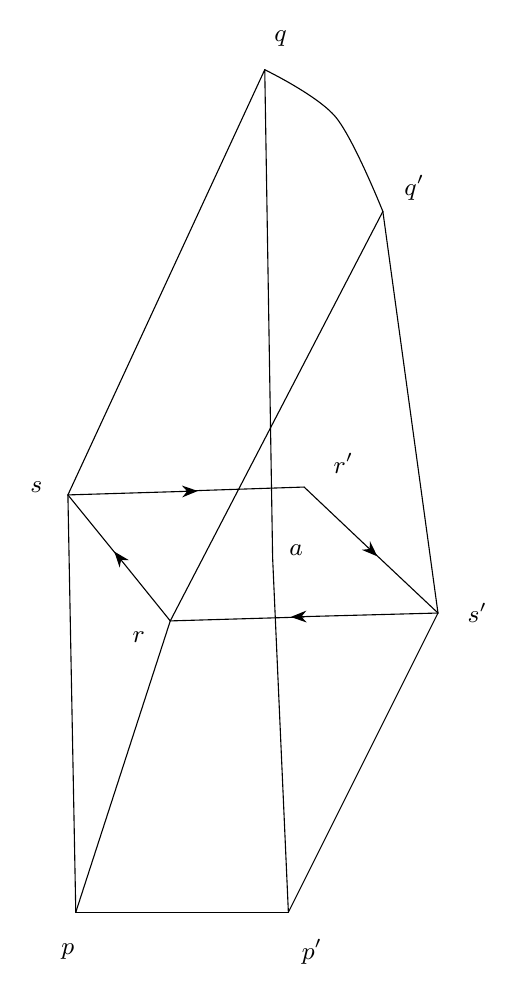
\begin{tikzpicture}[x=1mm,y=1mm,line cap=round,line join=round,font=\scriptsize]
\draw plot[smooth, tension=0.55] coordinates {(68,-13) (77,-19) (83,-31)};
\draw (68,-13) -- (43,-67);
\draw (68,-13) -- (69,-75);
\draw (83,-31) -- (90,-82);
\draw (83,-31) -- (56,-83);
\draw (43,-67) -- (44,-120);
\draw (56,-83) -- (44,-120);
\draw (90,-82) -- (71,-120);
\draw (69,-75) -- (71,-120);
\draw (44,-120) -- (71,-120);
\draw[-{Stealth[length=2mm]}] (43,-67) -- (59.5,-66.5);
\draw[-{Stealth[length=2mm]}] (73,-66) -- (82.3,-74.8);
\draw[-{Stealth[length=2mm]}] (90,-82) -- (71.3,-82.5);
\draw[-{Stealth[length=2mm]}] (56,-83) -- (48.9,-74.2);
\draw (58,-66.5) -- (73,-66);
\draw (81.5,-74) -- (90,-82);
\draw (73,-82.5) -- (56,-83);
\draw (49.5,-75) -- (43,-67);
\node[inner sep=1pt] at (70,-9) {\small $q$};
\node[inner sep=1pt] at (87,-28) {\small $q'$};
\node[inner sep=1pt] at (39,-66) {\small $s$};
\node[inner sep=1pt] at (78,-63) {\small $r'$};
\node[inner sep=1pt] at (95,-82) {\small $s'$};
\node[inner sep=1pt] at (52,-85) {\small $r$};
\node[inner sep=1pt] at (72,-74) {\small $a$};
\node[inner sep=1pt] at (43,-125) {\small $p$};
\node[inner sep=1pt] at (74,-125) {\small $p'$};
\end{tikzpicture}
\end{document}
